\documentclass[11pt,letterpaper]{article}
\usepackage[margin=1in]{geometry}
\usepackage{graphicx}
\usepackage{hyperref}
\usepackage{listings}
\usepackage{amsmath}
\pagestyle{headings}
\usepackage{epstopdf}

\begin{document}

\title{PHY 410 \\ Final Assignment}
\author{Han Wen \\ \tiny Person No. 50096432}
\date{\today}

\maketitle

\begin{abstract}
Final project for PHY 410, 2014 fall semester


\end{abstract}

\tableofcontents

\newpage
\section{Problem 1}

\subsection{Description}
Problem 1 (25 points). Consider a rocket of total mass $m_0$, with a mass
of $m_1$ when it is empty of propellant. Assume the rocket expels propellent at
a constant exhaust velocity $v_e$, and the mass linearly decreases with time
with rate B until it is spent :
$$
m(t)=max(m_1,m_0-Bt)
$$

Consider the “Saturn V” rocket with $m_0 = 2, 970, 000 kg$ and $m_1 = 130, 000
kg$ after the first stage, which can apply 34,020 kN of force to move
(“thrust”). The burn time is 165 s. This burn time corresponds to B = 17212
kg/s.
\url{http://en.wikipedia.org/wiki/Saturn_V}

a. (5 points) In the absence of air resistance, calculate the escape
  velocity off the surface of the earth if a rocket is fired straight up. 

b. (10 points) The “balle” program from Lecture 20 handles projectile
      motion in a gravitational field, close to the surface of the earth. Modify
       the “balle” program from Lecture 20 to account for the changing mass
          of a rocket, and the full gravitational potential from the earth for
         arbitrary radius. Plot the distance from the surface of the earth r(t), as
        well as the velocity v(t), as a function of time for the first stage of the
         Saturn V rocket. Does the rocket achieve escape velocity like this? 

c. (10 points) Now consider air resistance in the same problem. Imagine
 that the cross-sectional area of the rocket is $25m^2$, and that the density
of air (in $kg/m^3$ ) is equal to $\rho{(h)} = 1.2 e^{-h/h_0}$

 where h is the height off the earth’s surface in meters,
  and $h_0 = 10000 m$. With the same initial parameters as in (b),
 compare the results from (b) to the case with air resistance.


\subsection{Solution}

\subsubsection{PART a}
The condition for the rocket to just escape will be the total energy is 0, therefore:
$$
\frac{1}{2}mv^2=\frac{GMm}{r} \longrightarrow v=\sqrt{\frac{2GM}{r}}  
\longrightarrow v=11180.5m/s
$$
The m, M, r, G are mass of rocket, mass of earth, radius of earth, gravitational constant.


\subsubsection{PART b}


The code is included in the appendix, the result plot is shown below: Fig. ~\ref{figure1}

\begin{figure}
\begin{center}
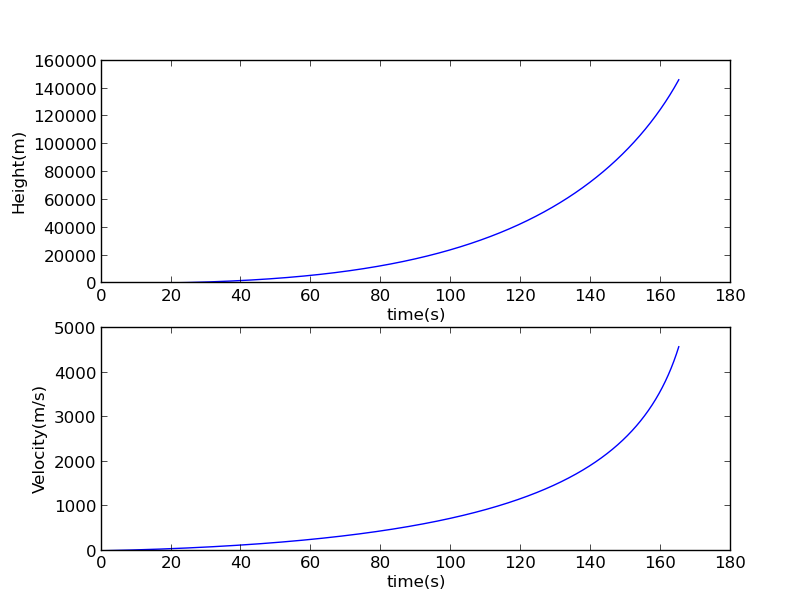
\includegraphics[width=0.8\linewidth,angle=0]{p1b.png}
\caption{Height and velocity vs. time, no friction}
\label{figure1}
\end{center}
\end{figure}

The final speed is 4580.3m/s less than the escape velocity.


\subsubsection{PART c}
With the friction, the result is shown below:Fig. ~\ref{figure2}
\begin{figure}
\begin{center}
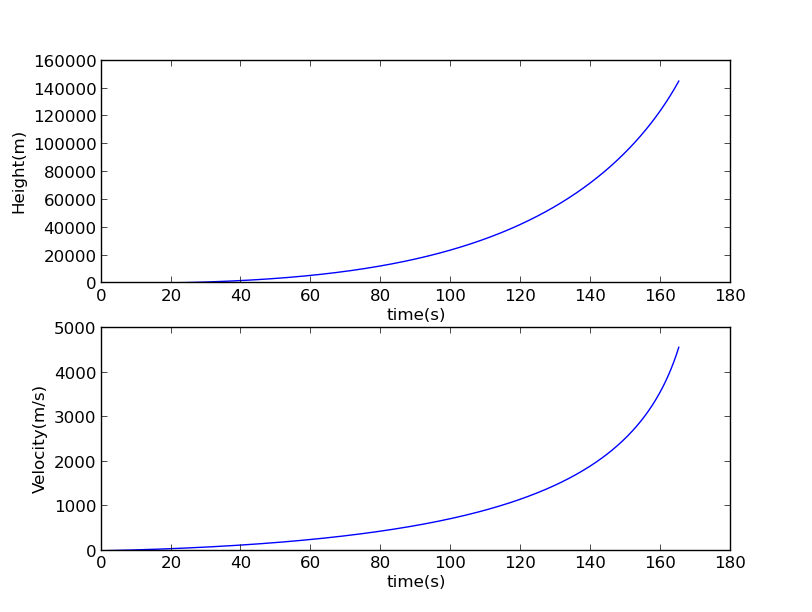
\includegraphics[width=0.8\linewidth,angle=0]{p1c.png}
\caption{Height and velocity vs. time, no friction}
\label{figure2}
\end{center}
\end{figure}



The final speed is 4567.3 m/s . We can see the results are almost the same, that's because when speed is high, the drag coefficient is no longer a constant, and will increase \cite{drag}. This program is only to show I can perform the calculation.





\section{Problem 2}
\subsection{Description}
Problem 2 (25 Points). In Kerbal Space Program (KSP),
orbital mechanics are simplified using a “patched” 2-body
approach, rather than solving the full N-body problem. That is,
the potential is a two-body gravitational potential, and only the
LARGEST gravitational force on the object is considered.
Assume you have a Saturn V (as in Problem 1) initially in a
circular orbit with an altitude of 100 km (this would correspond
to the third stage of the Saturn V rocket,
with m = 13500 kg). Assume you can apply a
maneuver in negligible time, such that the
velocity is imparted as an impulse, with a final
imparted velocity of 8000 m/s. (This is in
addition to the orbital velocity of a rocket at an
altitude of 100 km.) (Apologies to Kerbal Space
Program https://kerbalspaceprogram.com. No Kerbals
were harmed in the making of this final exam. I think.)

a.(5 points) Write an expression for V(r)/m,
where V(r) is the potential acting on the
rocket, and m is the mass of the rocket, for both the “true” and
“patched” earth-moon-rocket systems. Compare the two graphically by
plotting V(r)/m for both cases in the line connecting the earth and
moon.
b.(5 points) Calculate the orbital velocity of the Saturn V rocket at an
altitude of 100 km.
c.(15 points) Modify the “planar3body” code in Lecture 22 to handle
BOTH the “true” earth-moon-rocket potential, and the KSP “patched”
potential. Code a “Moon encounter” for Saturn V, such that your rocket
is deflected by the Moon’s gravity (in real life, the astronauts would
then “burn retrograde” to slow down and be captured by the moon). Do
this for both the “true” and “patched” potentials. Plot the trajectory of
your “Moon shot”. 
Consider the earth to be at rest for this purpose (also be sure to
change the initial x3,y3,vx3,vy3 to be 0,0,0,0). 
HINT : It is easiest to work in coordinates with the earth at the origin,
and use units such that the radii and orbital angular velocity of the
moon are 1.0 and 2⇡, respectively.

\subsection{Solution}
\subsubsection{PART a}

The code is included in the appendix, and the result diagram is shown here: Fig. ~\ref{figure3}

\begin{figure}
\begin{center}
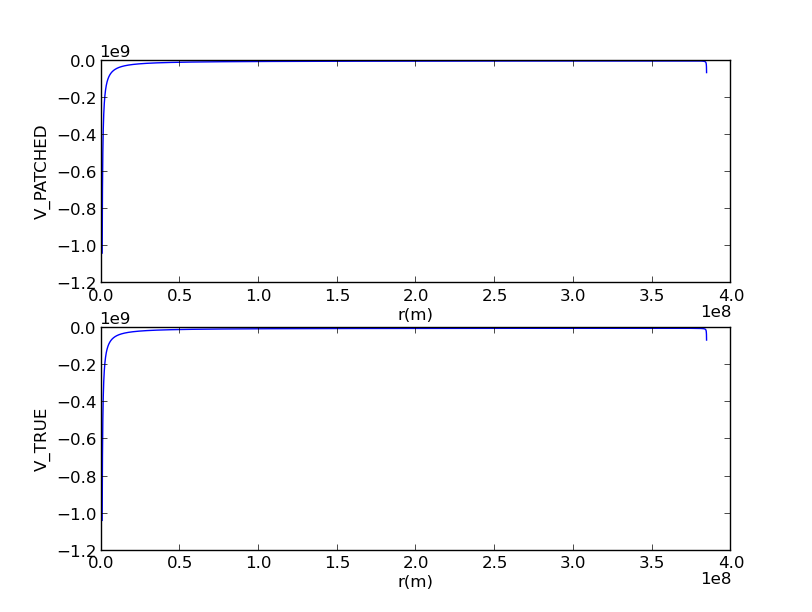
\includegraphics[width=0.8\linewidth,angle=0]{p2a.png}
\caption{real and patched potential for moon-earth-rocket system}
\label{figure3}
\end{center}
\end{figure}

\subsubsection{PART b}
$$
\frac{mv^2}{r}=\frac{GMm}{r^2} 
\longrightarrow\; v=\sqrt{\frac{GM}{r}}
v=7847.1 m/s
$$

\subsubsection{PART c}

I modified my code so that the radii and angular velocity of moon is 1.0 and $2\pi$. For simplicity, I chose the x coordinate of moon to be 0 and y to be 0.1592. The x and y coordinate for rocket to be -0.00268 , 0.0. 
For patched potential, the plot is shown here: Fig ~\ref{figure4} 

\begin{figure}
\begin{center}
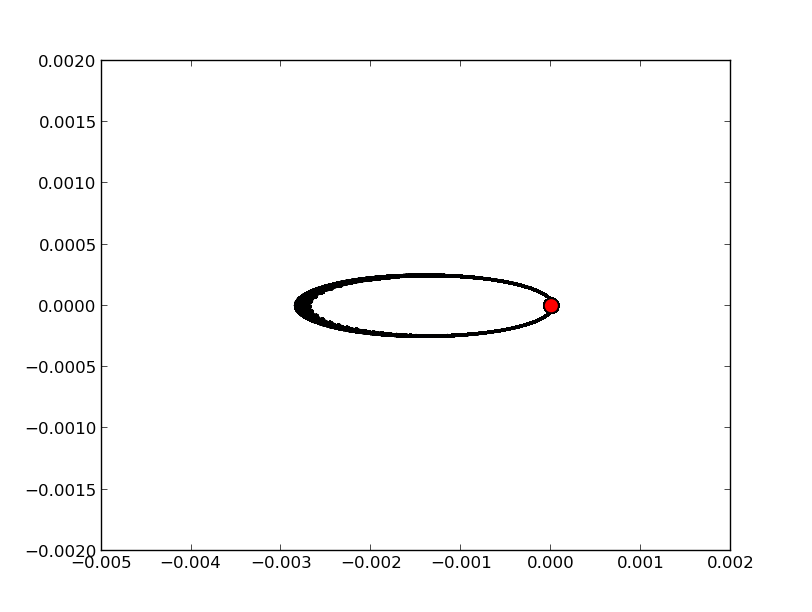
\includegraphics[width=0.8\linewidth,angle=0]{p2c_patched.png}
\caption{trajectory for patched potential for moon-earth-rocket system}
\label{figure4}
\end{center}
\end{figure}

For real potential, the plot is here: Fig. ~\ref{figure5}

\begin{figure}
\begin{center}
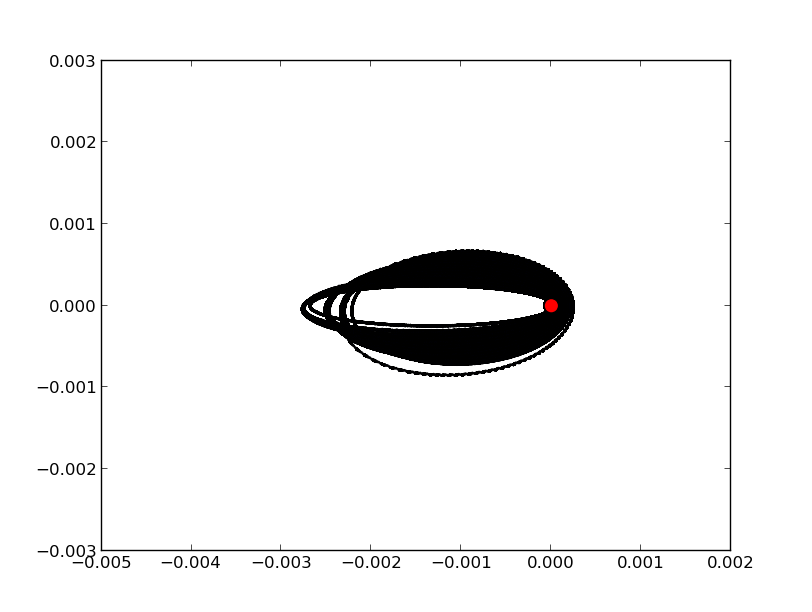
\includegraphics[width=0.8\linewidth,angle=0]{p2c_real.png}
\caption{trajectory for real potential for moon-earth-rocket system}
\label{figure5}
\end{center}
\end{figure}

We can see there is a little difference between two cases.



\section{Problem 3}
\subsection{Description}

\begin{figure}
\begin{center}
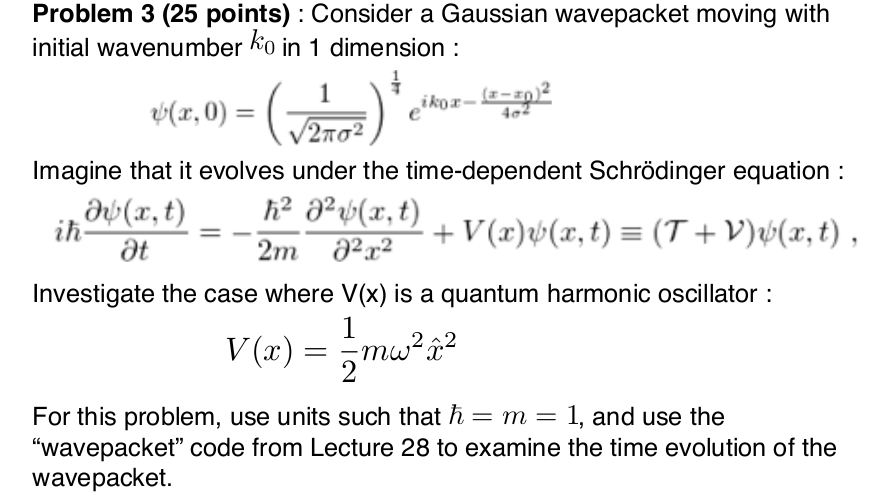
\includegraphics[width=0.8\linewidth,angle=0]{3a.png}
\label{figure6}
\end{center}
\end{figure}

\begin{figure}
\begin{center}
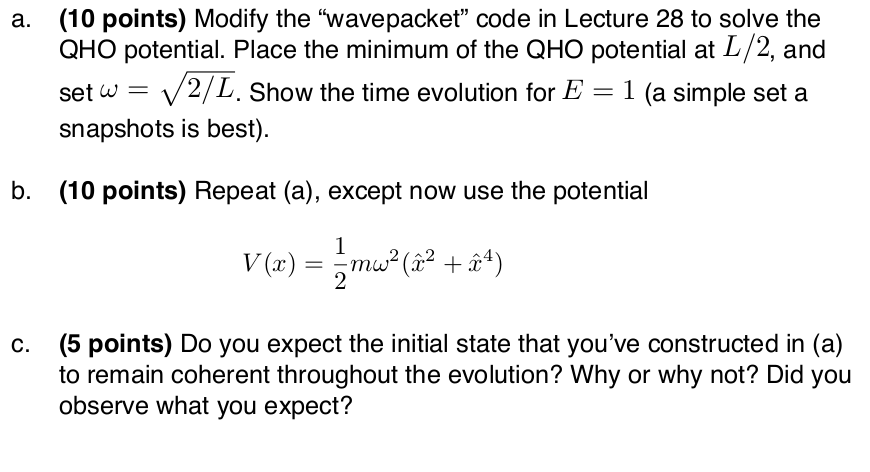
\includegraphics[width=0.8\linewidth,angle=0]{3b.png}
\label{figure7}
\end{center}
\end{figure}


\subsection{Solution}

\subsubsection{PART a}

The snapshots for the quantum harmonic oscillation is shown below: Fig. ~\ref{figure8}




\begin{figure}
\begin{center}
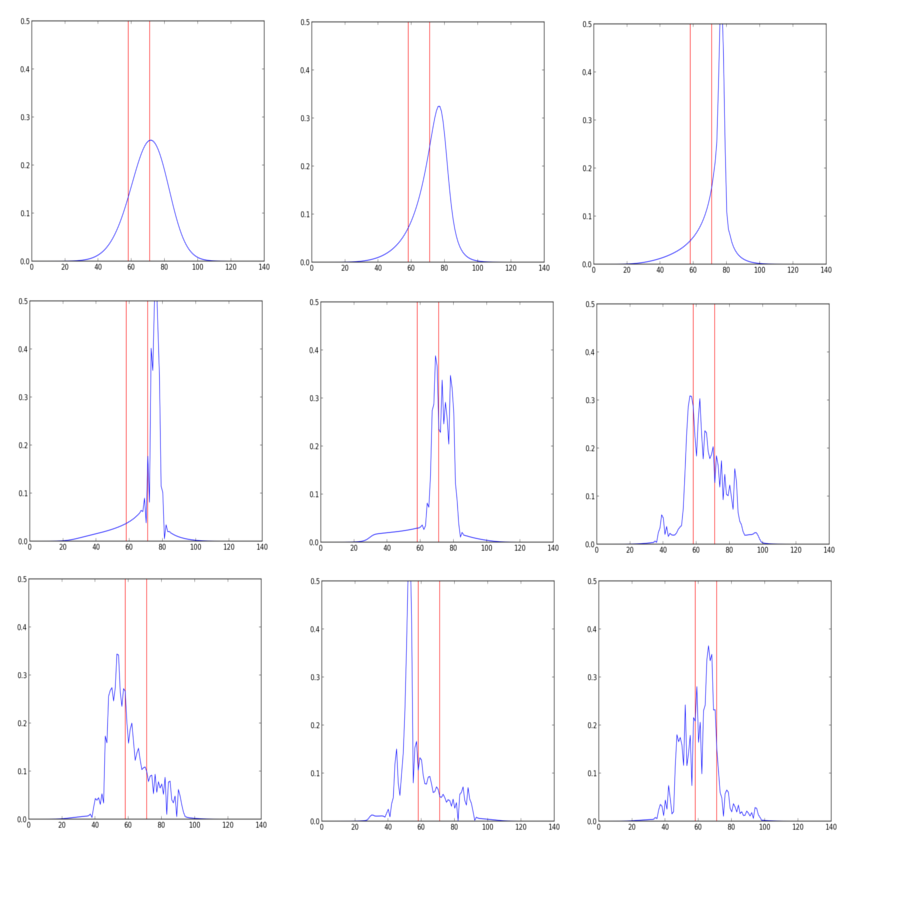
\includegraphics[width=0.8\linewidth,angle=0]{p32.png}
\caption{snapshots for quantum harmonic oscillation}
\label{figure8}
\end{center}
\end{figure}
\subsubsection{PART b}

The snapshots for this potential is shown below: Fig. ~\ref{figure9}

\begin{figure}
\begin{center}
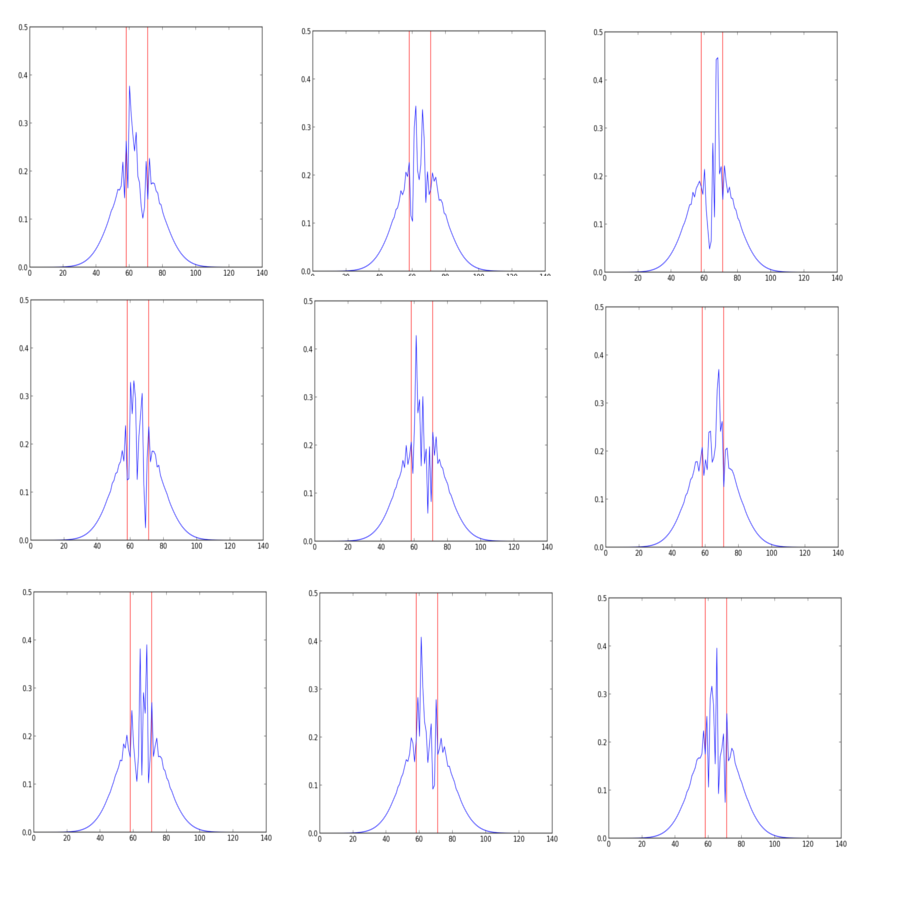
\includegraphics[width=0.8\linewidth,angle=0]{p324.png}
\caption{snapshots for specific potential}
\label{figure9}
\end{center}
\end{figure}


\subsubsection{PART c}
They should remain coherent. Because for a coherent state, during the evolution in time, the only change will be in its coefficient $e^{-i\omega{t}}$, therefore should remain coherent. The simulation support this, showing a same width of the wavepacket through out the evolution.


\section{Problem 4}
\subsection{Description}
Problem 4 (25 points). Consider the MC integration of a Gaussian
distribution with the Metropolis algorithm (“metropolis” code in Lecture 31).
a. (15 points) Modify the “metropolis” program to perform Metropolis
      integrations with the same number (A) for both the number of trials (M)
     and the number of Metropolis steps (N). Check the values of A = 5, 10,
    50, 100, 500, 1000, and report the accuracy of the answer (variable
   “ans”, compared to the true value). Perform this 5 times and report the
      average deviation for each choice of A.
b. (10 points) At what point do you achieve accuracy within 10% of the
  true answer? If you had to change either M or N (but not both) by a
 factor of two to achieve better accuracy, which would you do? Why?
Support your case with examples from the code.
\subsection{Solution}
\subsubsection{PART a}

Here is the table of my result: \ref{table1}

I used delta = 1


\begin{table}[h]
\caption{Result for different A\label{table1}}
\begin{tabular}{l l l}
\hline
 \textbf{number of A } & \textbf{Result}& \textbf{Deviation}\\
\hline
5	&$	0.771	\pm	0.112	$&	0.315	\\
5	&$	0.532	\pm	0.072	$&	0.173	\\
5	&$	0.985	\pm	0.073	$&	0.421	\\
5	&$	0.296	\pm	0.051	$&	0.11	\\
5	&$	0.44	\pm	0.067	$&	0.119	\\
average of 5	&$	0.6048	\pm	0.075	$&	0.2276	\\
10	&$	0.699	\pm	0.051	$&	0.195	\\
10	&$	1.879	\pm	0.123	$&	0.482	\\
10	&$	0.93	\pm	0.074	$&	0.384	\\
10	&$	1.003	\pm	0.083	$&	0.224	\\
10	&$	0.816	\pm	0.073	$&	0.204	\\
average of 10	&$	1.0654	\pm	0.0808	$&	0.2978	\\
50	&$	0.994	\pm	0.023	$&	0.066	\\
50	&$	0.93	\pm	0.02	$&	0.075	\\
50	&$	0.939	\pm	0.021	$&	0.065	\\
50	&$	1.082	\pm	0.024	$&	0.072	\\
50	&$	0.875	\pm	0.021	$&	0.056	\\
average of 50	&$	0.964	\pm	0.0218	$&	0.0668	\\
100	&$	1.069	\pm	0.013	$&	0.044	\\
100	&$	0.975	\pm	0.012	$&	0.039	\\
100	&$	0.958	\pm	0.012	$&	0.037	\\
100	&$	0.919	\pm	0.011	$&	0.041	\\
100	&$	1.018	\pm	0.013	$&	0.047	\\
average of 100	&$	0.9878	\pm	0.0122	$&	0.0416	\\
500	&$	1.002	\pm	0.003	$&	0.009	\\
500	&$	1.003	\pm	0.003	$&	0.009	\\
500	&$	0.992	\pm	0.003	$&	0.01	\\
500	&$	0.985	\pm	0.003	$&	0.009	\\
500	&$	1.002	\pm	0.003	$&	0.01	\\
average of 500	&$	0.9968	\pm	0.003	$&	0.0094	\\
1000	&$	1.003	\pm	0.001	$&	0.005	\\
1000	&$	1.006	\pm	0.001	$&	0.005	\\
1000	&$	1.005	\pm	0.001	$&	0.005	\\
1000	&$	1.004	\pm	0.001	$&	0.005	\\
1000	&$	1.004	\pm	0.001	$&	0.004	\\
average of 1000	&$	1.0044	\pm	0.001	$&	0.0048	\\
\hline
\end{tabular}
\end{table}





\subsubsection{PART b}

I modified the code(included in the appendix) to try 100 trials for each M and N, see if any of those trial have accuracy lower than 10-percent. Turned out, although the random nature make this result only a statistical one, A = 20 would be a ideal number. 

I think changing N will be a better idea. Because N is the number for each round of M, if change M, the each individual cycle still gives a result with large error, the total average will not improve as efficient as changing N, which improve the individual result for M cycle.

When using 500 for both M,N, the result is $1.0039\pm0.0027$
When changing M to 1000, the result is $1.0031\pm0.0019$
When changing N to 1000, the result is $1.0019\pm0.0019$

Apparently changing N is more effective. Although one trial won't be representative enough, choosing a big number should help improve the result.  

Also I repeat the code for 10-percent with either M or N times 2, the result showed the biggest number for M times 2 is bigger. Indicating changing N is more effective

\newpage
\section*{Acknowledgements}

I discussed this assignment with my classmates and used material from the
cited references, but this write-up is my own.

\begin{thebibliography}{9}


\bibitem{coursepage}
PHY 410-505 Webpage, \url{http://www.physics.buffalo.edu/phy410-505}.



\bibitem{drag}
Wiki for air resistance
\url{http://en.wikipedia.org/wiki/Drag_%28physics%29}


\end{thebibliography}


\newpage

\appendix
\section{Appendix}

\subsection{python code}

The following python code was used to obtain the results in this report:

\lstinputlisting[language=python]{rocket.py}

\lstinputlisting[language=python]{planar3body.py}

\lstinputlisting[language=python]{twopotential.py}

\lstinputlisting[language=python]{wavepacket.py}

\lstinputlisting[language=python]{pbmetropolis.py}

\end{document}
